\section{Microprocesador simple}
En esta sección se verá como interconectar los dispositivos vistos en la sección anterior para
realizar un microprocesador sencillo en VHDL. Para ello se describirá brevemente algunos conceptos
genéricos del microprocesador a implementar.

\subsection{Computadora sencilla}
Un diseño tradicional de la arquitectura interna de una computadora consiste en tres unidades 
principales, el procesador (CPU), las memorias donde guardar el programa y los datos, 
y un módulo de entrada salida para comunicarnos con el exterior.
La figura \ref{arquitectura} esquematiza estos tres módulos interconectados por dos buses
principales, uno de direcciones y otro de datos, adicionalmente existirán lineas de control 
para indicar el flujo de la información entre dichos módulos.

\begin{figure}[h]
  \centering
    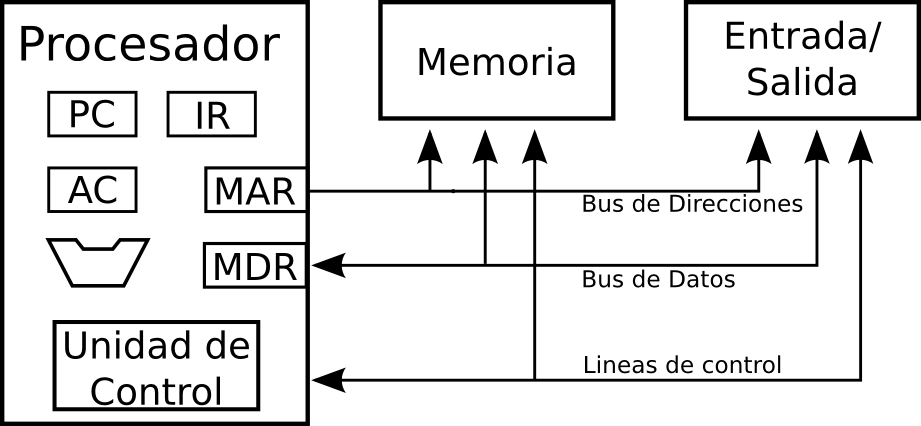
\includegraphics[width=.8\textwidth]{graficos/computadora.png}
  \caption{Arquitectura de una computadora simple}
  \label{arquitectura}
\end{figure}

Internamente el procesador contiene varios registros para almacenar datos dentro del
procesador. Algunos registros será visibles para el usuario como el Acumulador (AC) y el 
Program Counter (PC). Mientras que otros servirán para manejo interno:

\begin{itemize}
 \item MAR (Memory Addres Register): Este registro contiene la dirección del dato que se 
 quiere leer o escribir. El registro está conectado con el bus de direcciones, y su contenido se refleja en este bus.
 \item MDR (Memory Data Register): El registro está conectado al bus de datos y a través de él, 
 el CPU lee o escribe un dato a dicho bus.
 \item IR (Instruction Register): Después de que se ha obtenido una instrucción de la memoria, la CPU lo 
 almacena en este registro.
\end{itemize}

\subsection{Instrucciones y programas}
Para el desarrollo del microprocesador se define un formato de instrucción como el que se observa en 
la figura \ref{instruction}

\begin{figure}[h]
  \centering
    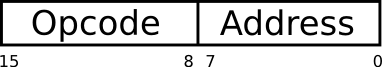
\includegraphics[width=.3\textwidth]{graficos/instruccion.png}
  \caption{Formato de la instrucción}
  \label{instruction}
\end{figure}

El set de instrucciones que implementaremos es básico (4 instrucciones), se describe en la tabla 
\ref{set_instruccion}

\begin{table}[!hbt] 
\centering
\begin{tabular}{|l|l|c|}
\hline
 \textbf{Mnemonico} & \textbf{Operación} & \textbf{OpCode}\\ \hline
ADD dirección & AC $\Leftarrow$ AC + contenido de la dirección de memoria & 00\\ \hline
STORE dirección& contenido de la dirección de memoria $\Leftarrow$ AC & 01\\ \hline
LOAD dirección& AC $\Leftarrow$ contenido de la dirección de memoria & 02\\ \hline
JUMP dirección& PC $\Leftarrow$ dirección & 03 \\ \hline
JNEG dirección& Si AC < 0 entonces PC $\Leftarrow$ dirección & 04 \\ \hline
\end{tabular}
  \caption{Set de instrucciones}
  \label{set_instruccion}
\end{table}

\subsection{Ciclos de ``Fetch'', ``Decode'', ``Execute''}
Normalmente las instrucciones se dividirán en varias etpas de instrucción, que llamaremos
``Fetch, Decode y Execute'' (F-D-E) respectivamente.
El ciclo F-D-E es el período que tarda un CPU en ejecutar una instrucción en código de máquina. 
El procesador captura (``fetch'') una instrucción de memoria, la decodifica (``decode``) 
para determinar que operando requiere y luego la ejecuta (''execute'').

La implementación del ciclo de F-D-E requiere algunas transferencias de registros y ciclos de reloj.

La figura \ref{fde} describe las acciones a realizar en cada etapa.

\begin{figure}[h]
  \centering
    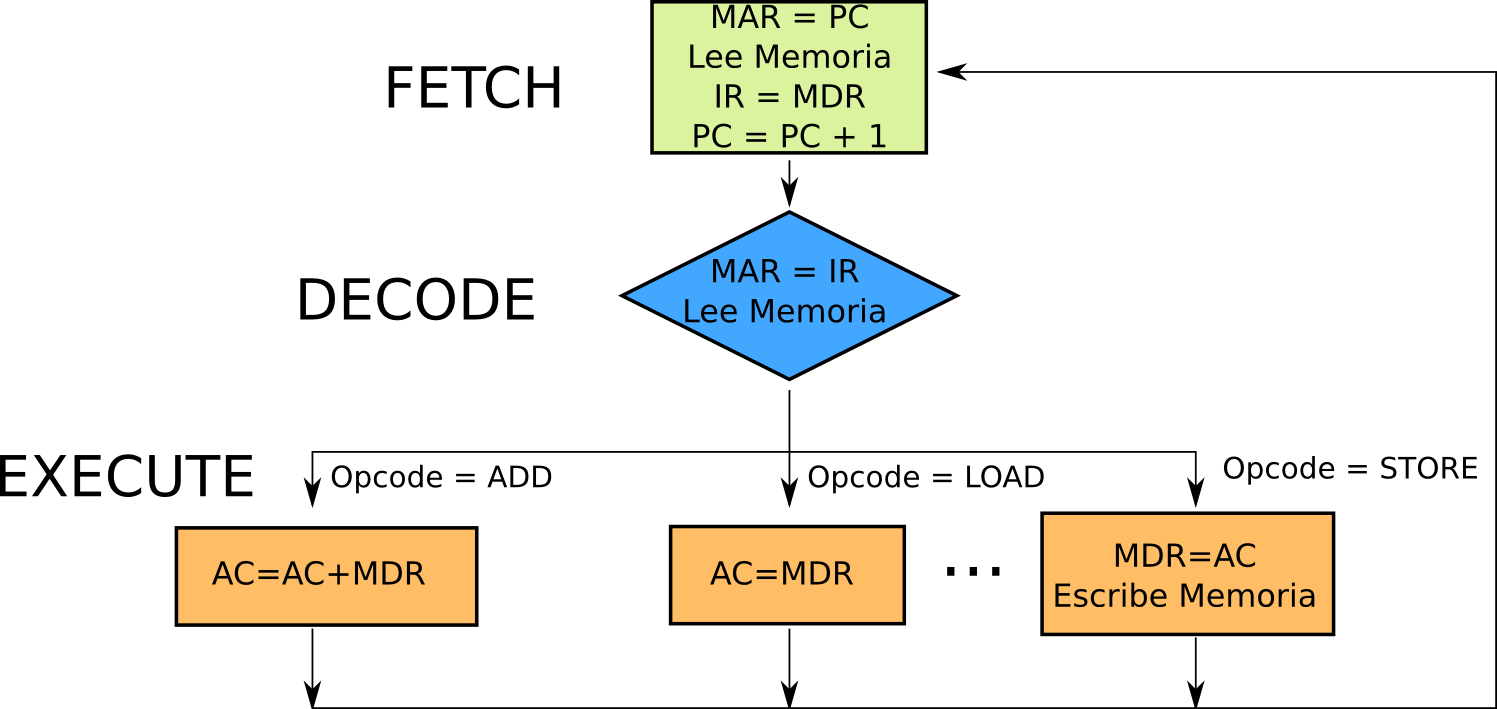
\includegraphics[width=1\textwidth]{graficos/fde.png}
  \caption{Ciclo de Fetch, Decode y Execute}
  \label{fde}
\end{figure} 

El ``Program Counter'' (PC) tiene la dirección de la instrucción actual. Normalmente para captar la próxima
instrucción de memoria el procesador deberá incrementar el PC. 
El registro de direcciones de memoria (MAR) se deberá actualizar con el PC de la instrucción que se captará.

\subsection{Modelo en VHDL}

memoria.vhd:
\begin{lstlisting}[style=vhdl, basicstyle=\footnotesize\ttfamily]
LIBRARY IEEE;
USE IEEE.STD_LOGIC_1164.ALL;
USE IEEE.STD_LOGIC_ARITH.ALL;
USE IEEE.STD_LOGIC_UNSIGNED.ALL;
ENTITY memory IS
  PORT( read_data     : OUT STD_LOGIC_VECTOR( 15 DOWNTO 0 );
        read_address  : IN STD_LOGIC_VECTOR( 7 DOWNTO 0 );
        write_data    : IN STD_LOGIC_VECTOR( 15 DOWNTO 0 ); 
        write_address : IN STD_LOGIC_VECTOR( 7 DOWNTO 0 );
        Memwrite      : IN STD_LOGIC;
        Clock         : IN STD_LOGIC );
  END memory;

ARCHITECTURE behavior OF memory IS
                --Define un nuevo tipo de datos de arreglo de memoria
  TYPE memory_type IS ARRAY ( 0 TO 255 ) OF STD_LOGIC_VECTOR( 15 DOWNTO 0 );
  SIGNAL memory: memory_type;
BEGIN
  --Lee la memoria y convierte el indice del arreglo a entero mediante CONV_INTEGER
  read_data <= memory( CONV_INTEGER( read_address( 7 DOWNTO 0 ) ) ) ;
  PROCESS       --Escritura de memoria
  BEGIN
    WAIT UNTIL clock 'EVENT AND clock = '1';
    IF ( memwrite = '1' ) THEN
                   --Convierte el indice del arreglo a entero mediante CONV_INTEGER
      memory( CONV_INTEGER( write_address( 7 DOWNTO 0 ) ) ) <= write_data;
    END IF;
  END PROCESS;
END behavior;
\end{lstlisting}

uprocesador.vhd:
\begin{lstlisting}[style=vhdl, basicstyle=\footnotesize\ttfamily]
LIBRARY IEEE;
USE IEEE.STD_LOGIC_1164.ALL;
USE IEEE.STD_LOGIC_ARITH.ALL;
USE IEEE.STD_LOGIC_UNSIGNED.ALL;

ENTITY SCOMP IS 
PORT( clock, reset  : IN STD_LOGIC;
      program_counter_out : OUT STD_LOGIC_VECTOR( 7 DOWNTO 0 );
      register_AC_out : OUT STD_LOGIC_VECTOR(15 DOWNTO 0 );
      memory_data_register_out : OUT STD_LOGIC_VECTOR(15 DOWNTO 0 ));
END SCOMP;

ARCHITECTURE up OF scomp IS
TYPE STATE_TYPE IS ( reset_pc, fetch, decode, execute_add, execute_load, 
execute_store, execute_store3, execute_store2, execute_jump );
SIGNAL state: STATE_TYPE;
SIGNAL instruction_register, memory_data_register : STD_LOGIC_VECTOR(15 DOWNTO 0 );
SIGNAL register_AC : STD_LOGIC_VECTOR(15 DOWNTO 0 );
SIGNAL program_counter : STD_LOGIC_VECTOR( 7 DOWNTO 0 );
SIGNAL memory_address_register : STD_LOGIC_VECTOR( 7 DOWNTO 0 );
SIGNAL memory_write : STD_LOGIC;

                      --Instanciacion de memoria (256 16-bit words)
  COMPONENT memory
    PORT( read_data     : OUT STD_LOGIC_VECTOR( 15 DOWNTO 0 );
          read_address  : IN STD_LOGIC_VECTOR( 7 DOWNTO 0 );
          write_data    : IN STD_LOGIC_VECTOR( 15 DOWNTO 0 ); 
          write_address : IN STD_LOGIC_VECTOR( 7 DOWNTO 0 );
          Memwrite      : IN STD_LOGIC;
          Clock         : IN STD_LOGIC );
  END COMPONENT;

  BEGIN
    memory_256: memory
           PORT MAP( read_data      => memory_data_register,
                     read_address   => memory_address_register,
                     write_data     => register_AC , 
                     write_address  => memory_address_register,
                     Memwrite       => memory_write,   
                     Clock          => clock);

    program_counter_out       <= program_counter;
    register_AC_out           <= register_AC;
    memory_data_register_out  <= memory_data_register;


                      --Estados

PROCESS ( CLOCK, RESET )
  BEGIN
  IF reset = '1' THEN
    state <= reset_pc;
  ELSIF clock'EVENT AND clock = '1' THEN
    CASE state IS
                  --Reseteo de la computadora, necesario para limpiar los registros                  
    WHEN reset_pc =>
        program_counter         <= "00000000";
        memory_address_register <= "00000000";
        register_AC             <= "0000000000000000";
        memory_write            <= '0';
        state                   <= fetch;
                  --Capta la instruccion de memoria y suma 1 al PC
    WHEN fetch =>
        instruction_register    <= memory_data_register;
        program_counter         <= program_counter + 1;
        memory_write            <= '0';
        state                   <= decode;        
                  --Decodifica la instruccion y envia la direccion del operando
    WHEN decode =>
        memory_address_register <= instruction_register( 7 DOWNTO 0);
        CASE instruction_register( 15 DOWNTO 8 ) IS
              WHEN "00000000" =>
                state <= execute_add;
              WHEN "00000001"=>
                state <= execute_store;
              WHEN "00000010" =>
                state <= execute_load;
              WHEN "00000011"=>
                state <= execute_jump;
              WHEN OTHERS =>
                state <= fetch;
        END CASE;
                  --Ejecuta la instruccion ADD
    WHEN execute_add =>
      register_ac             <= register_ac + memory_data_register;
      memory_address_register <= program_counter;
      state                   <= fetch;
                  --Ejecuta la instruccion STORE
                  --(necesita tres ciclos de clock)
    WHEN execute_store =>
      memory_write  <='1';
      state         <= execute_store2;
                  --Este estado asegura que la direccion de memoria
                  --es valida hasta despues que memory_write se desactiva
    WHEN execute_store2 =>
      memory_write  <= '0';
      state         <= execute_store3;
    WHEN execute_store3 =>  memory_address_register <= program_counter;
      state         <= fetch;
                  --Ejecuta la instruccion LOAD
    WHEN execute_load =>
      register_ac             <= memory_data_register;
      memory_address_register <= program_counter;
      state                   <= fetch;
                  --Ejecuta la instruccion JUMP
    WHEN execute_jump =>  
      memory_address_register <= instruction_register( 7 DOWNTO 0 );
      program_counter         <= instruction_register( 7 DOWNTO 0 );
      state                   <= fetch;
    WHEN OTHERS =>
      memory_address_register <= program_counter;
      state                   <= fetch;
    END CASE;
  END IF;
  END PROCESS;
END up;
\end{lstlisting}
\subsection{Simulaciones}
Para realizar la simulación, haremos un cálculo sencillo que se implementará en la memoria:


\lstset{language={[x86masm]Assembler}}
\begin{lstlisting}[basicstyle=\footnotesize\ttfamily]
 LOAD A  ;Cargo el primer valor de $11
 ADD B   ;Sumo el contenido de $11 a $12
 STORE C ;Guardo el resultado en $10
\end{lstlisting}
\lstset{language=vhdl}

Para cargar el programa en la memoria generaremos un archivo
binario con los opcodes del programa anterior e inicializaremos las
direcciones de memoria 0x11 y 0x12. El archivo ``memoria.mem'' 
quedará, por lo tanto, como se observa en la figura \ref{uprocmemoria}

\begin{figure}[h!]
  \centering
    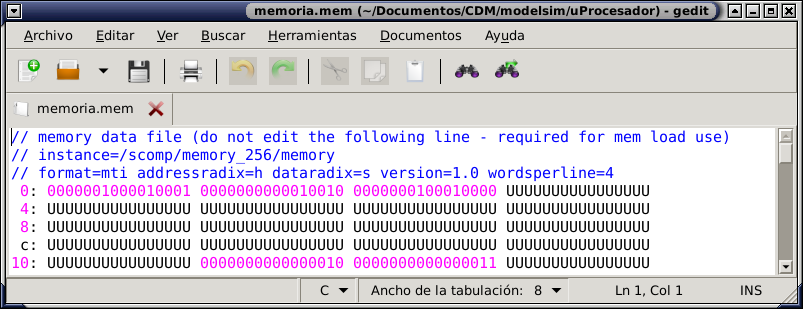
\includegraphics[width=1\textwidth]{graficos/memoria_uproc.png}
  \caption{Estructura del archivo ``memoria.mem''}
  \label{uprocmemoria}
\end{figure}

Como se observa en la simulación de la figura \ref{msuprocesador}, luego de que baja la señal de 
``Reset'', la señal ``State'' comienza con el estado ``reset'', luego pasa a ``Fetch'', ``Decode'' 
y ``Execute'' para las tres instrucciones. El program counter avanza de la posición ``0x00'' hasta
la ``0x03''. Cuando se produce el estado ``Execute\_store2'', se activa la señal de escritura en memoria.

\begin{figure}[h!]
  \centering
    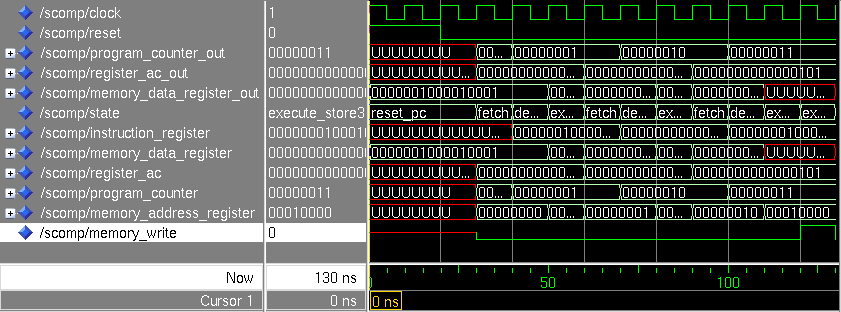
\includegraphics[width=1\textwidth]{graficos/uprocesador.png}
  \caption{Simulación del procesador}
  \label{msuprocesador}
\end{figure}

Luego de la ejecución del código la memoria queda con la información de la figura \ref{mempostsimulation}.

\begin{figure}[h!]
  \centering
    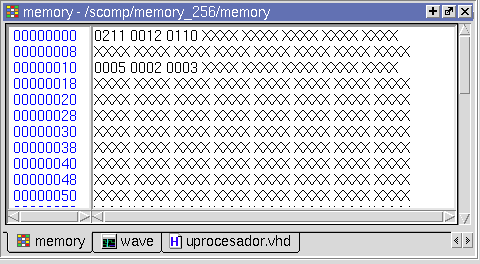
\includegraphics[width=.6\textwidth]{graficos/uprocpostsimulation.png}
  \caption{Estado de la memoria luego de la simulación}
  \label{mempostsimulation}
\end{figure}

\newpage

\subsection{Implementación}
A continuación se describirán algunos detalles de la implementación en la FPGA.

El procesador desarrollado hasta ahora es muy sensillo y no posee ninguna unidad de depuración para ingresar el código a depurar. Por lo
tanto a la hora de realizar la implementación, nos encontraremos con la dificultad de escribir el código en la memoria.

Herramientas como Quartus de Altera o ISE de Xilinx, poseen herramientas para inicializar directamente la memoria ram. Para utilizar estas herramientas 
necesitariamos implementar por lo menos un controlador de memoria.

Como el objetivo de este tutorial es implementar un procesador sensillo, se propone una solución de implementación que es independiente
del fabricante de FPGA (herramientas IDE) cómo de la arquitectura del circuito que se utilizará.
La técnica consiste en preinicializar sectores del vector de memoria con los valores que se desean escribir de la siguiente manera:

memoria.vhd:
\begin{lstlisting}[style=vhdl, basicstyle=\footnotesize\ttfamily]

  PROCESS       --Escritura de memoria
  BEGIN
  process(reset,clock,memwrite) begin
    if reset='1' then
	  memory(0) <= x"0211";
	  memory(1) <= x"0012";
	  memory(2) <= x"0110";
	  memory(3) <= x"0302";
	  memory(11) <= x"0002";
	  memory(12) <= x"0003";
     for i in 13 to 255 loop 
	    memory(i) <= x"0000";
		 end loop;
  .....
  end process;
\end{lstlisting}
